% 荷质比的测定
%汤姆孙测电子荷质比的方法|磁聚焦法

\subsection{荷质比}
原理:利用电子(或其他带电粒子)在磁场中偏转性的特点,测得粒子电荷与质量之比(即荷质比)
说明:荷质比是带电微观粒子的基本参量之一.

典型的测量荷质比的方式有两种

\subsection{汤姆孙测量电子荷质比的方法}

\begin{figure}[ht]
\centering
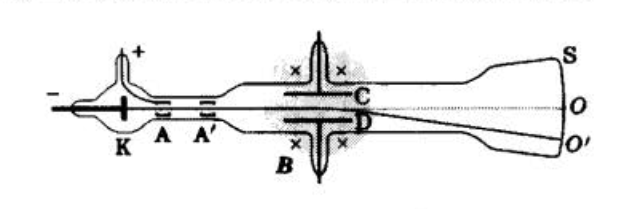
\includegraphics[width=7cm]{./figures/Charge1.png}
\caption{汤姆孙法测荷质比} \label{Charge_fig1}
\end{figure}

\subsection{磁聚焦法}

\begin{figure}[ht]
\centering
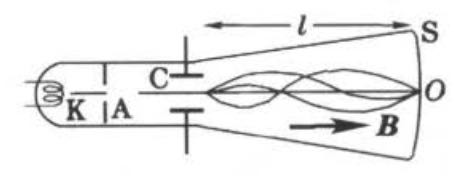
\includegraphics[width=7cm]{./figures/Charge2.png}
\caption{磁聚焦法测荷质比} \label{Charge_fig2}
\end{figure}

抽真空的玻璃管中装有热阴极K和有小孔的阳极 $A$.在 $A$,$K$ 之间加电压 $\Delta U$ 时,由阳极的小孔射出的电子动能为:
\begin{equation}
1/2mv^2=e\Delta U
\end{equation}
从而我们得到其速率为:
\begin{equation}
v=\sqrt{2e\Delta U/m}
\end{equation}
在电容器 $C$ 上加一个不大的横向交变电场,使不同时刻通过这里的电子发生不同程度的偏转.在电容器 $C$ 和荧光屏 $S$ 之间加一均匀的纵向磁场.

%待继续编辑
